\documentclass[12pt,a4paper]{article}
\usepackage[utf8]{inputenc}
\usepackage[T1]{fontenc}
\usepackage{amsmath}
\usepackage{amsfonts}
\usepackage{amssymb}
\usepackage{amsthm}
\usepackage{graphicx}
\usepackage{subfigure}
\usepackage{float}
\newtheorem*{lemma}{Lemma}
\newtheorem*{theorem}{Theorem}
\newtheorem*{prf}{\textbf{Proof}}
\usepackage{caption}
\DeclareMathOperator{\n}{\nabla}
\DeclareMathOperator{\E}{\mathrm{E}}
\DeclareMathOperator{\xyz}{\textbf{numpy.random.normal()}}
\title{CS331-HW5-Lukang-Sun}
\begin{document}
	\maketitle
	\paragraph{p1.}
		In my experiments(see Figure\ref{img1}.), I set $d = 2, n = 10,  f(x)=\frac{1}{ 10} \sum_{i=1}^{10} f_i(x), f_i(x) = \frac{1}{2}\left\|a_{i}^{} x-b_{i}\right\|_{2}^{2}$, $a = [matrix([[0.94884523, 0.31257516]]), matrix([[0.64695759, 0.79089169]]), \\matrix([[0.70218109, 0.91473775]]), matrix([[0.03035042, 0.21034799]]), \\matrix([[0.99278455, 0.2554682 ]]), matrix([[0.16064759, 0.09062056]]),\\ matrix([[0.41438167, 0.77718962]]), matrix([[0.4953842 , 0.93027311]]), \\matrix([[0.7692516 , 0.19772597]]), matrix([[0.12430258, 0.03779965]])],\\
		b = [matrix([[0.4231786]]), matrix([[0.524466]]), matrix([[0.17981303]]), matrix([[0.50033184]]),\\ matrix([[0.71116473]]), matrix([[0.0604399]]), matrix([[0.37100656]]), matrix([[0.91263449]]),\\ matrix([[0.66417151]]), matrix([[0.65995097]])]
		$, based on these information, we can get that $x_{\star} = matrix([[-0.54051746]
		[-0.26890662]])$, I sample 10 points in the last step to estimate $\mathrm{E}\left[||x_{\text{last step}}-x_{\star}||^2\right]$. As for baselines, I select full gradient descent and CGD with Sparsification($p=0.2$). 
	\begin{figure}
		\centering
		\subfigure[ ]{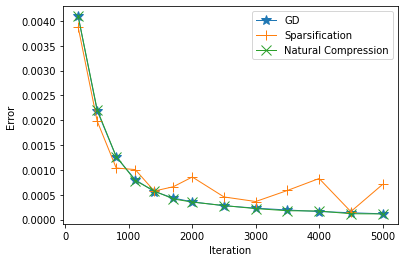
\includegraphics[width=6.7cm]{500.png}} 
		\subfigure[]{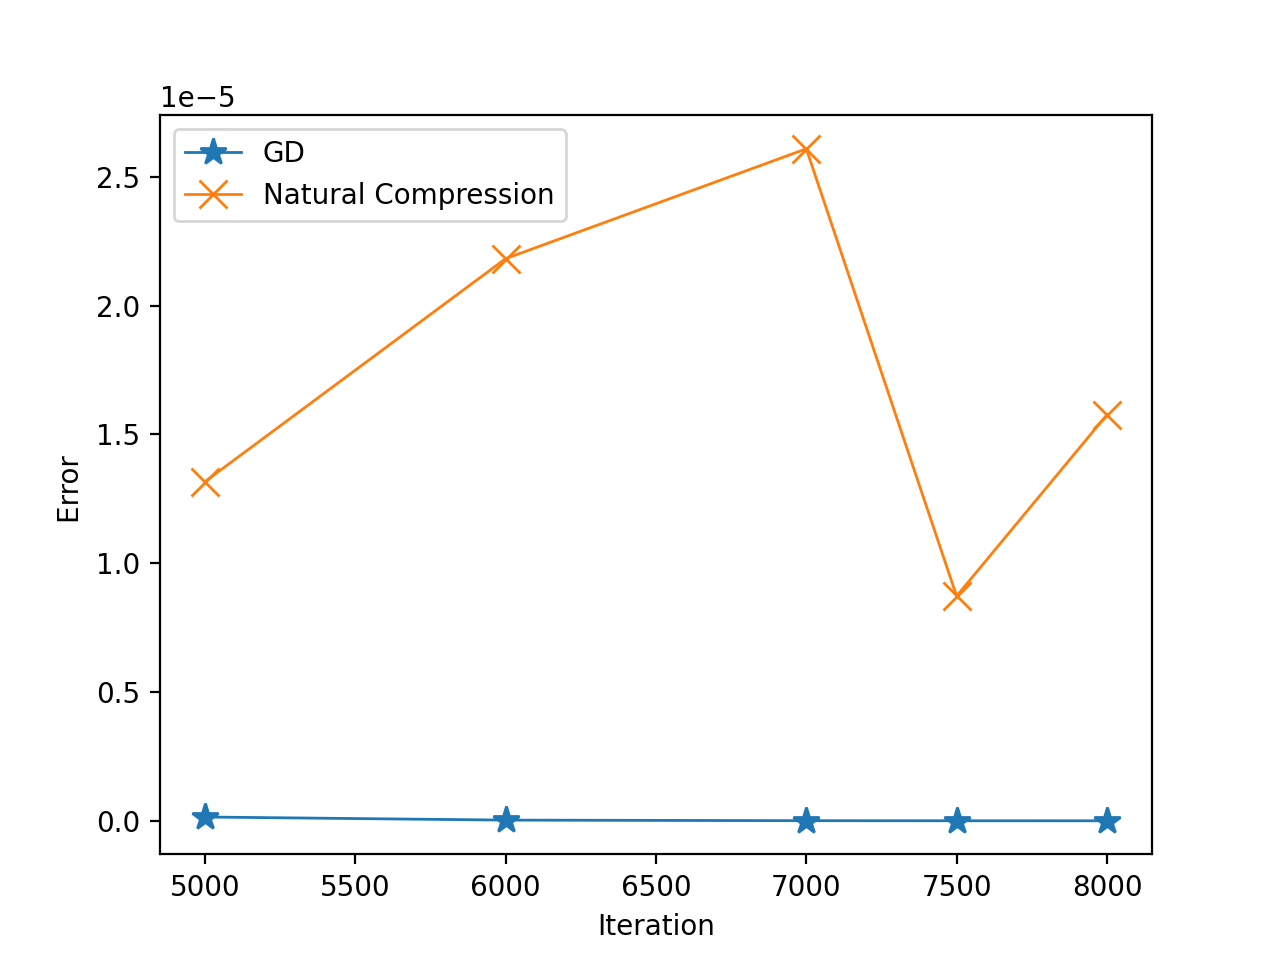
\includegraphics[width=6.7cm]{Figure_100_iter.png}}
		\\ %换行
		
		
		\caption{  The horizontal axis is iteration, vertical axis is the error. In (a), I set step  size as $1/500,$, you will see that 1000 steps, full gradient descent and DCGD with natural compression perform quite well, but CGD with sparsification will shake, this can be explained by sparsification operator has bigger $\omega$ than natural compression operator. In (b), you will see the difference between DCGD with natural compression and gradient descent, in which, the error of gradient descent keeps converging to 0, while, DCGD with natural compression will shake.} %图片标题
		\label{img1}
	\end{figure}
	
	
	
	\paragraph{p2.}
			In my experiments(see Figure\ref{img2}.), I set $d = 2, n = 10,  f(x)=\frac{1}{ 10} \sum_{i=1}^{10} f_i(x), f_i(x) = \frac{1}{2}\left\|a_{i}^{} x-b_{i}\right\|_{2}^{2}$, $a = [matrix([[0.94884523, 0.31257516]]), matrix([[0.64695759, 0.79089169]]), \\matrix([[0.70218109, 0.91473775]]), matrix([[0.03035042, 0.21034799]]), \\matrix([[0.99278455, 0.2554682 ]]), matrix([[0.16064759, 0.09062056]]),\\ matrix([[0.41438167, 0.77718962]]), matrix([[0.4953842 , 0.93027311]]), \\matrix([[0.7692516 , 0.19772597]]), matrix([[0.12430258, 0.03779965]])],\\
	b = [matrix([[0.4231786]]), matrix([[0.524466]]), matrix([[0.17981303]]), matrix([[0.50033184]]),\\ matrix([[0.71116473]]), matrix([[0.0604399]]), matrix([[0.37100656]]), matrix([[0.91263449]]),\\ matrix([[0.66417151]]), matrix([[0.65995097]])]
	$, based on these information, we can get that $x_{\star} = matrix([[-0.54051746]
	[-0.26890662]]),x_0=matrix([[-0.5]
	[-0.2]])$, I sample 10 points in the last step to estimate $\mathrm{E}\left[||x_{\text{last step}}-x_{\star}||^2\right]$. I set the compression operator on server as identity operator( means there is no compression). 
	\begin{figure}
		\centering
		\subfigure[ ]{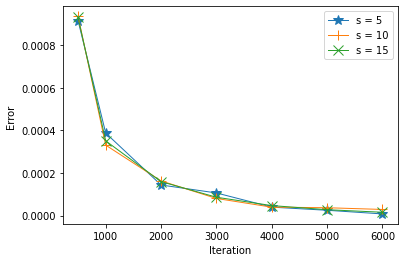
\includegraphics[width=6.7cm]{521.png}} 
		\subfigure[]{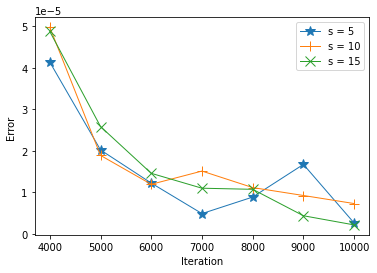
\includegraphics[width=6.7cm]{5 10 15 4000hou.png}}
		\\ %换行
		\subfigure[ ]{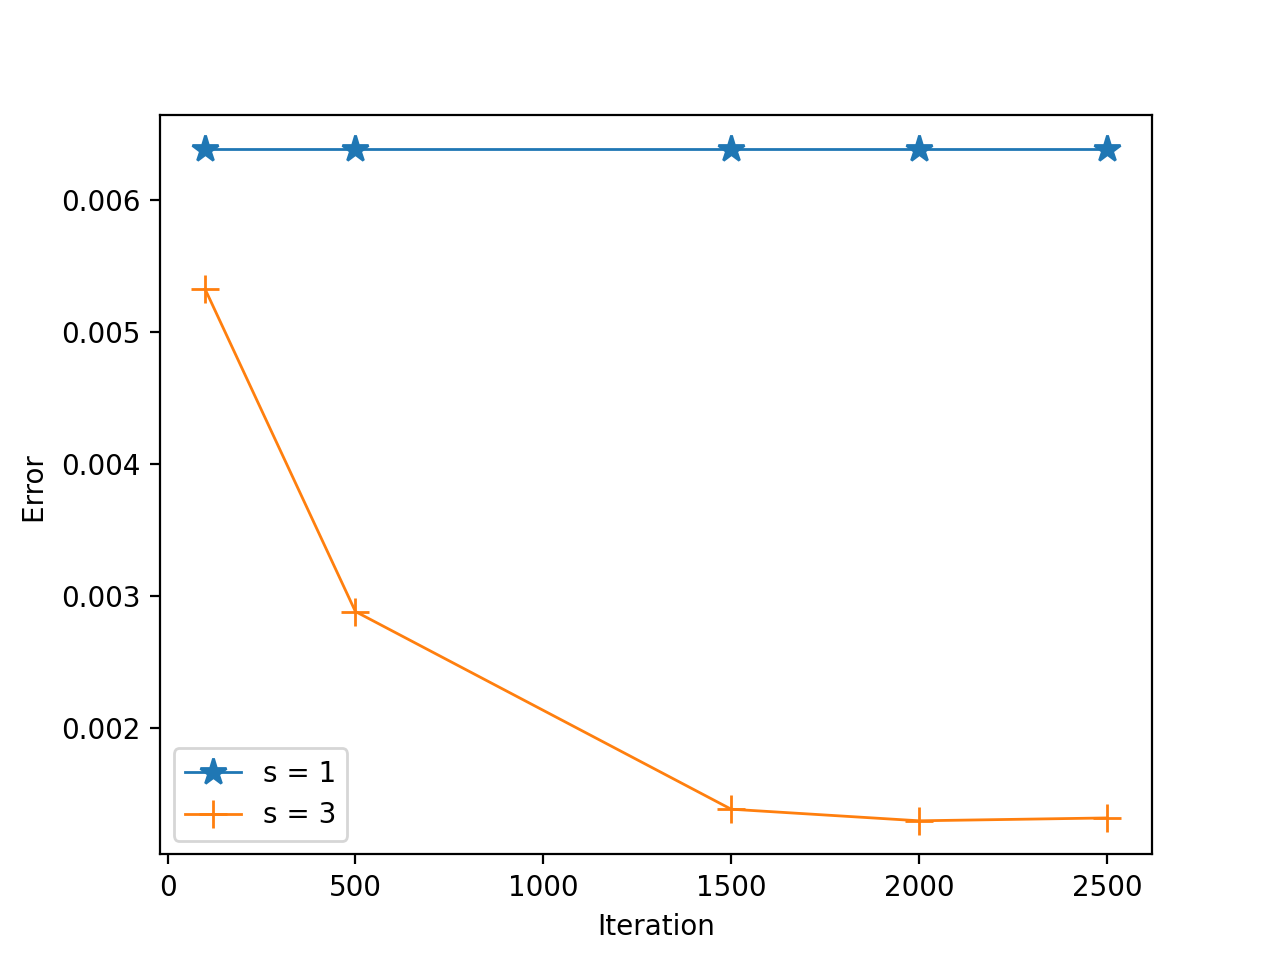
\includegraphics[width=6.7cm]{Figure_5 1 3 3000qian.png}} 
		\subfigure[]{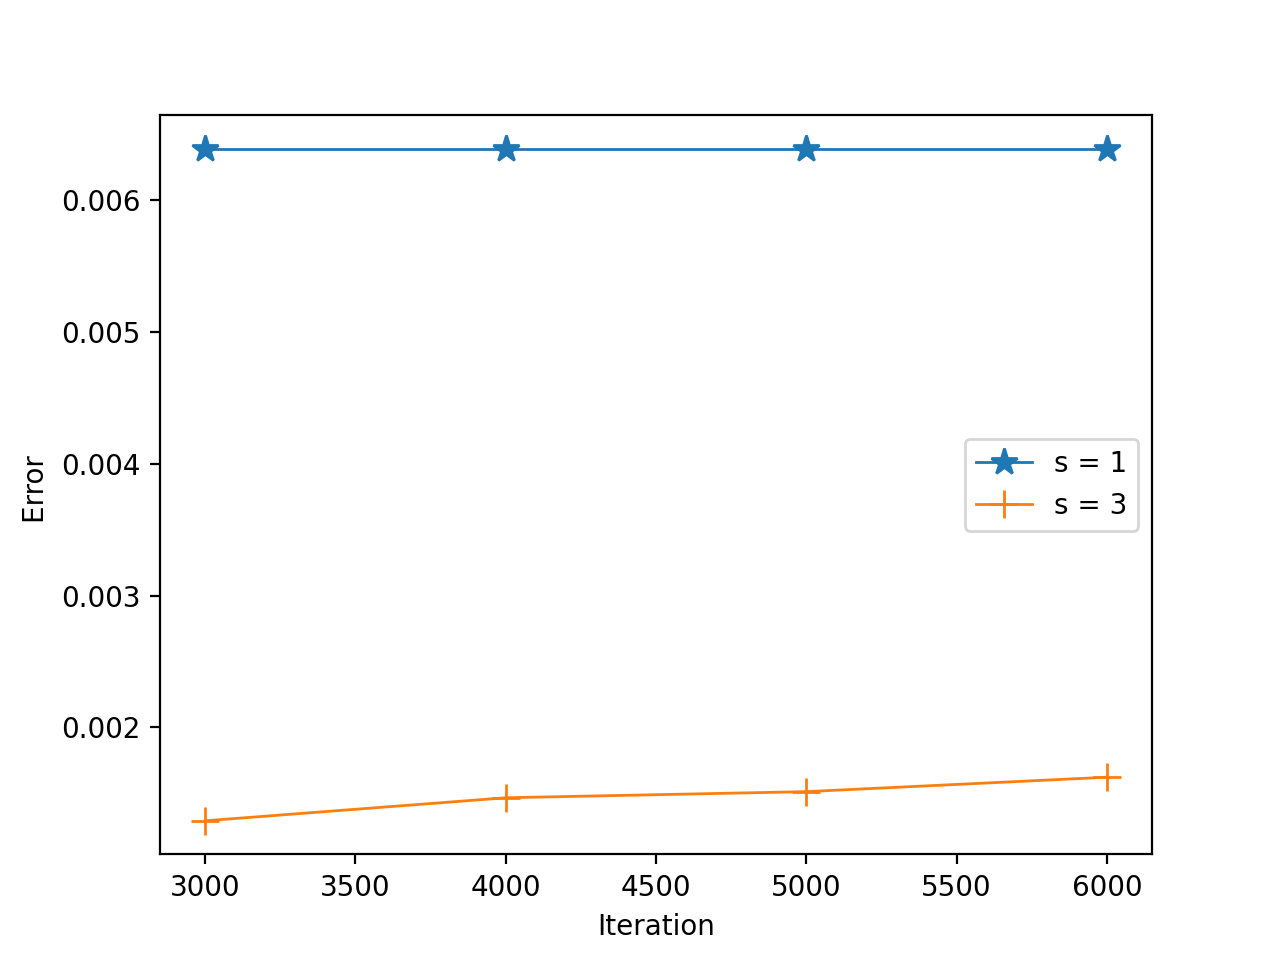
\includegraphics[width=6.7cm]{Figure_5 13.png}}
		\\ %换行
		\subfigure[ ]{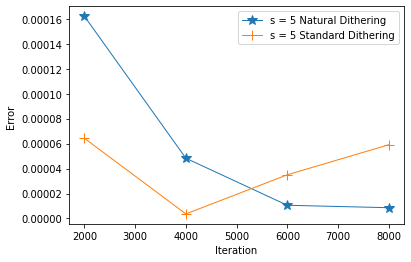
\includegraphics[width=6.7cm]{dither 2.png}} 
		\subfigure[]{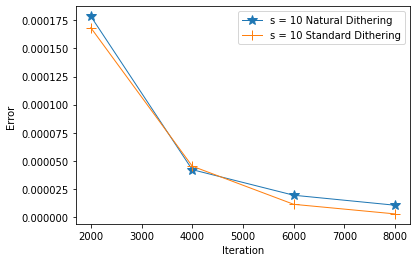
\includegraphics[width=6.7cm]{dither 10.png}}
		
		
		\caption{  The horizontal axis is iteration, vertical axis is the error.I set step  size as $1/500,$, in (a) and (b),you will see DCGD with natural dithering with $s = 5, 10, 15,$ are quite similar, actually the theory states that $\omega=\frac{1}{8}+\frac{d^{\frac{1}{r}}}{2^{s-1}} \min \left\{1, \frac{d^{\frac{1}{r}}}{2^{s-1}}\right\}$,for $s=5, 10, 15$, $\omega= \frac{1}{8}+ \text{term smaller than 1/16}$, they are very close. While in (c) and(d), I se t $s= 1,3$, actually for these two value of $s$, the corresponding $\omega$ are very different and you can also observe that from (c) and (d). In (e) and (f), I show the diffrence between natural dithering and standard dithering, when $s$ is big(like $s = 10$), the result(f) are similar, while $s$ small($s=5 $), you can observe the difference.} %图片标题
		\label{img2}
	\end{figure}
	
	
	
	\paragraph{p3.}	for (a) and (b), without loss of generality, we only consider when $d=1$.
	\textbf{(a)}
\begin{equation*}
	\E\left[\mathcal{C}_{int}(t)\right]=(t-\lfloor t\rfloor)(\lfloor t\rfloor +1)+(1-t+\lfloor t\rfloor)(\lfloor t\rfloor)=t
\end{equation*}	
\newline
\textbf{(b)} Let's take $t\in (0,1)$, then $\lfloor t\rfloor=0,\lfloor t\rfloor+1=1$,
\begin{equation*}
	\E\left[||\mathcal{C}_{int}(t)||^2\right]=(t-\lfloor t\rfloor)(\lfloor t\rfloor +1)^2+(1-t+\lfloor t\rfloor)(\lfloor t\rfloor)^2=(t-\lfloor t\rfloor)(\lfloor t\rfloor +1)+(1-t+\lfloor t\rfloor)(\lfloor t\rfloor)=t,
\end{equation*}
if $\mathcal{C}_{int}\in\mathbb{B}(\omega)$, this means $t\leq (\omega+1)t^2$, for any $t\in (0,1)$, this is impossible, since $1/t\mapsto +\infty,$ as $t\mapsto 0$.
\newline
\textbf{(c)}
\begin{equation*}
	\begin{aligned}
	\E\left[||\mathcal{C}_{int}(t)-t||^2\right]=&(t-\lfloor t\rfloor)(\lfloor t\rfloor +1-t)^2+(1-t+\lfloor t\rfloor)(\lfloor t\rfloor-t)^2\\
	&\overset{x:=t-\lfloor t\rfloor}{=}x(1-x)\leq \frac{1}{4},
	\end{aligned}
\end{equation*}
since $x\in [0,1)$, the maximum value of $x(1-x)$ is attained at $x=1/2$, which equals $1/4$. Above we only consider each component, for vector $x\in \mathbb{R}^d$, just take the summation for $i=1,\cdots,d$, we get the upper bound is $\frac{d}{4}$.
	\paragraph{p4.}	
	\begin{equation}
			||\text{Top}_k(x)-x||^2=\sum_{i=k+1}^{d}||x_{\pi_i}||^2
	\end{equation}
	\begin{equation}
		||x||^2=\sum_{i=1}^d||x_{\pi_i}||^2=k(\frac{1}{k})\sum_{i=1}^{k}||x_{\pi_i}||^2+(d-k)\frac{1}{d-k}\sum_{i=k+1}^d||x_{\pi_i}||^2
	\end{equation}
while due to the definition,
\begin{equation}
	\frac{1}{k}\sum_{i=1}^{k}||x_{\pi_i}||^2\geq\frac{1}{d-k}\sum_{i=k+1}^d||x_{\pi_i}||^2,
\end{equation}
so by (2) and (3), we know
\begin{equation}
	||x||^2\geq \frac{d}{d-k}\sum_{i=k+1}^d||x_{\pi_i}||^2\overset{\text{(1)}}{=}\frac{d}{d-k}||\text{Top}_k(x)-x||^2,
\end{equation}
which proves the exercise.

	
	
	
\end{document}